\documentclass[12pt]{article}

\usepackage[utf8]{inputenc}
\usepackage[danish]{babel}
\usepackage{latexsym, amsfonts, amssymb, amsthm, amsmath, siunitx, graphicx, pgfplots}
\usepackage[hidelinks]{hyperref}
\usepackage{sagetex}

\sisetup{exponent-product = \cdot,
  output-decimal-marker = {,}}

%Giles Castelles incfig
\usepackage{import}
\usepackage{xifthen}
\usepackage{pdfpages}
\usepackage{transparent}

\newcommand{\incfig}[2][1]{%
  \def\svgwidth{#1\columnwidth}
  \import{../figures/}{#2.pdf_tex}
}

\pdfsuppresswarningpagegroup=1

\setlength{\parindent}{0in}
\setlength{\oddsidemargin}{0in}
\setlength{\textwidth}{6.5in}
\setlength{\textheight}{8.8in}
\setlength{\topmargin}{0in}
\setlength{\headheight}{18pt}

\pgfplotsset{compat=newest}

\pgfplotsset{every axis/.append style={
  axis x line=middle,    % put the x axis in the middle
  axis y line=middle,    % put the y axis in the middle
  axis line style={<->,color=black}, % arrows on the axis
}}

\title{Opgaver til forelæsning 14}
\author{Noah Rahbek Bigum Hansen}
\date{DATO}

\begin{document}

\maketitle

\section*{Opg. 9.35}

\begin{figure} [ht]
  \centering
  \caption{}
  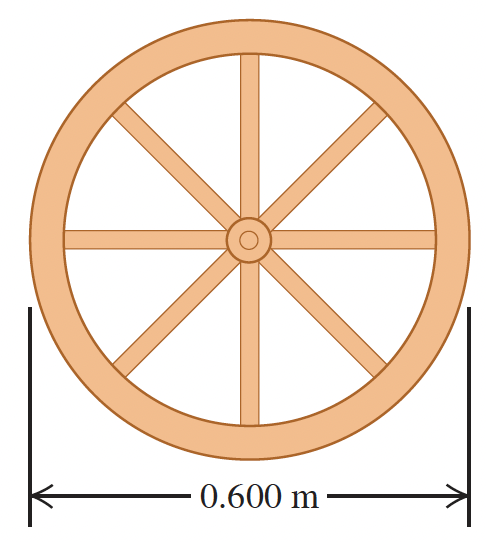
\includegraphics[width=0.3\linewidth]{../figures/E9_35.png}
  \label{fig:E9_35}
\end{figure}

A wagon wheel is constructed as shown in (\textbf{\autoref{fig:E9_35}}). The radius of the wheel is \qty{0,300}{m}, and the rim has mass \qty{1,40}{kg}. Each of the eight spokes that lie along a diameter and are \qty{0,300}{m} long has mass \qty{0,280}{kg}. What is the moment of inertia of the wheel about an axis through its center and perpendicular to the plane of the wheel?
\bigbreak
Vi modellerer kanten af hjulet som en hul cylinder og denne har derfor et inertimoment om den pågældende akse på
\[
I_{kant} = MR^2 = \qty{1,40}{kg}\cdot (\qty{0,300}{m})^2 = \qty{0,126}{kg\cdot m^2}
,\] 
og de 8 eger modelleres som tynde pinde med rotationsakse om en af sine ender. Disse har hver et inertimoment på
\[
  I_{ege} = \frac{1}{3}ML^2 = \frac{1}{3} \qty{0,280}{kg}\cdot (\qty{0,300}{m})^2 = \qty{0,0084}{kg\cdot m^2}
.\] 
Og altså bliver hjulets samlede inertimoment
\[
I_{tot} = I_{kant} + 8I_{ege} = \qty{0,126}{kg\cdot m^2} + 8\cdot \qty{0,0084}{kg\cdot m^2} = \qty{0,1932}{kg\cdot m^2}
.\] 

\section*{Opg. 9.49}

\begin{figure} [ht]
  \centering
  \caption{}
  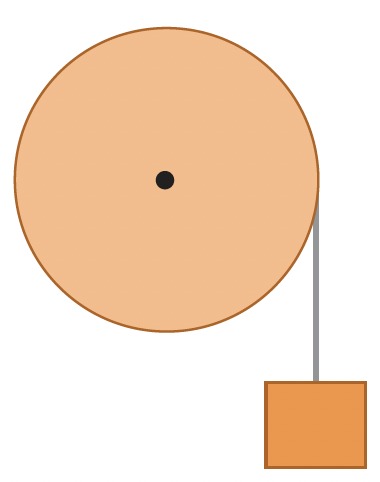
\includegraphics[width=0.3\linewidth]{../figures/E9_49.png}
  \label{fig:E9_49}
\end{figure}

A thin, light wire is wrapped around the rim of a wheel (\textbf{\autoref{fig:E9_49}}). The wheel rotates without friction about a stationary horizontal axis that passes through the center of the wheel. The wheel is a uniform disk with radius $R = \qty{0,280}{m}$. An object of mass $m = \qty{4,20}{kg}$ is suspended from the free end of the wire. The system is released from rest and the suspended object descends with constant acceleration. If the suspended object moves downward a distance of \qty{3,00}{m} in \qty{2,00}{s}, what is the mass of the wheel?
\bigbreak
Det antages at det udelukkende er tyngdekraften, der påvirker blokken. Først findes hastigheden som blokken falder med
\[
x = \frac{1}{2}v\cdot t \implies v_x = \frac{2x}{t} = \frac{2\cdot \qty{3,00}{m}}{\qty{2,00}{s}} = \qty{3}{\frac{m}{s}}
.\] 
Vi antager at systemet er tabsfrit. Altså har vi
\[
  k_1 + U_1 = k_2 + U_2 \implies m\cdot g\cdot x = \frac{1}{2}m\cdot v_x^2 + \frac{1}{2}I\cdot \omega^2
.\] 
Vi kan lave følgende omskrivning
\[
\frac{1}{2}\cdot I\cdot \omega^2 = \frac{1}{2}\cdot \frac{1}{2}MR^2 \cdot  \frac{v_x^2}{R^2} = \frac{1}{4}\cdot Mv_x^2
.\] 
Dermed fås at
\[
  m\cdot g\cdot x = \frac{1}{2}\cdot m\cdot v_x^2 + \frac{1}{4}Mv_x^2 \implies M = \frac{4 \left( m\cdot g\cdot x - \frac{1}{2}m\cdot v_x^2 \right)}{v_x^2}
.\] 
Og altså har vi at
\[
  M = \frac{4 \left( \qty{4,20}{kg}\cdot \qty{9,81}{\frac{m}{s^2}\cdot \qty{3,00}{m}} - \frac{1}{2} \qty{4,20}{kg}\cdot (\qty{3,00}{\frac{m}{s^2}})^2 \right) }{(\qty{3,00}{\frac{m}{s}})^2} = \qty{46,5}{kg}
.\]


\section*{Opg. 9.57}
A slender rod with length $L$ has a mass per unit length that varies with distance from the left end, where $x = 0$, according to $\frac{\mathrm{d}m}{\mathrm{d}x} = \gamma x$, where $g$ has units of \unit{kg/m^2}.


\subsection*{(a)}
Calculate the total mass of the rod in terms of $\gamma$ and $L$.
\bigbreak
For at finde pindens masse integreres over pindens længde
\[
\int_m  \mathrm{d}m = \gamma \int_0^L x \mathrm{d}x = \frac{1}{2}\gamma L^2 
.\] 

\subsection*{(b)}
Use Eq. (9.20) to calculate the moment of inertia of the rod for an axis at the left end, perpendicular to the rod. Use the expression you derived in part (a) to express $I$ in terms of $M$ and $L$. How does your result compare to that for a uniform rod? Explain.
\bigbreak
Eq. (9.20) lyder
\[
I = \int r^2 \, \mathrm{d}m
.\] 
Altså har vi at
\[
I = \gamma \int_0^L x^3 \, \mathrm{d}x = \frac{1}{4}\gamma L^4 = \frac{1}{2}ML^2
.\]
For en jævntfordelt pind ville inertimomentet være $I = \frac{1}{3}ML^2$.

\subsection*{(c)}
Repeat part (b) for an axis at the right end of the rod. How do the results for parts (b) and (c) compare? Explain.
\bigbreak
Her har vi i stedet at
\[
\mathrm{d}m = \gamma\left( L-x \right) \, \mathrm{d}x
.\] 
Det vises hurtigt at massen er den samme, hvilket også giver fin logisk mening
\[
M = \gamma \int L-x \, \mathrm{d}x  = \gamma \left[ Lx - \frac{1}{2}x^2 \right]_0^L = \frac{1}{2}\gamma L^2 
.\] 
Dermed bliver inertimomentet
\[
I = \gamma \int_0^L x^2(L-x) \, \mathrm{d}x = \gamma \int_0^L Lx^2-x^3 \, \mathrm{d}x = \gamma \left[ \frac{1}{3}Lx^3 - \frac{1}{4}x^4 \right]_0^{L} = \frac{1}{12}\gamma L^4 = \frac{1}{6}ML^2 
.\] 
Det giver god mening at inertimomentet i dette tilfælde er mindre idet størstedelen af massen nu er placeret tættere på omdrejningsaksen.

\section*{Opg. 9.79}

\begin{figure} [ht]
  \centering
  \caption{}
  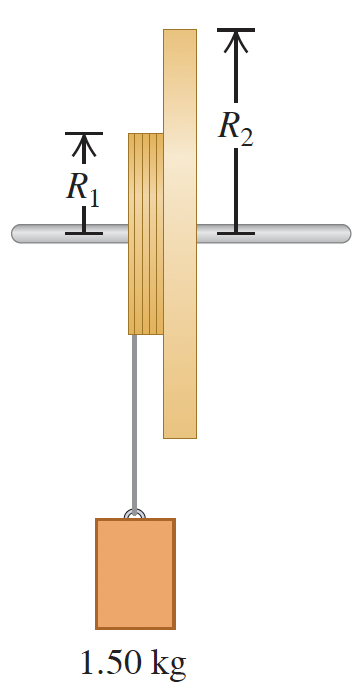
\includegraphics[width=0.25\linewidth]{../figures/P9_79.png}
  \label{fig:P9_79}
\end{figure}

Two metal disks, one with radius $R_1 = \qty{2,50}{cm}$ and mass $M_1 = \qty{0,80}{kg}$ and the other with radius $R_2 = \qty{5,00}{cm}$ and mass $M_2 = \qty{1,60}{kg}$, are welded together and mounted on a frictionless axis through their common center (\textbf{\autoref{fig:P9_79}}).


\subsection*{(a)}
What is the total moment of inertia of the two disks?
\bigbreak
De to diske antages hver især at have jævn massefordeling og de modelleres som to solide cylindre. Inertimomentet af en solid cylinder er generelt givet ved
\[
I = \frac{1}{2}MR^2 
.\]
Altså får vi at
\[
  I_{tot} = \frac{1}{2}\qty{0,80}{kg}\cdot \qty{2,50}{cm} + \frac{1}{2}\qty{1,60}{kg}\cdot \qty{5,00}{cm} = \qty{2,50e-3}{kg\cdot m^2}
.\] 

\subsection*{(b)}
A light string is wrapped around the edge of the smaller disk, and a \qty{1,50}{kg} block is suspended from the free end of the string. If the block is released from rest at a distance of \qty{2,00}{m} above the floor, what is its speed just before it strikes the floor?
\bigbreak
Konservation af energi giver os at
\[
k_1+U_1=k_2+U_2 \implies msg = \frac{1}{2}m\cdot v^2 + \frac{1}{2}I\omega^2 = \frac{1}{2}mv^2 + \frac{1}{2}I\left( \frac{v}{R_1} \right)^2
.\]
\[
v_1 = \sqrt{\frac{2msg}{m + \frac{I}{R_1^2}}} = \sqrt{\frac{2\cdot \qty{1,50}{kg}\cdot \qty{2,00}{m}\cdot \qty{9,81}{\frac{m}{s^2}}}{\qty{1,50}{kg} + \frac{\qty{2,50e-3}{kg\cdot m^2}}{(\qty{2,50e-2}{m})^2}}} = \qty{5,80}{\frac{m}{s}} 
.\] 


\subsection*{(c)}
Repeat part (b), this time with the string wrapped around the edge of the larger disk. In which case is the final speed of the block greater? Explain.
\bigbreak
\[
v_2 = \sqrt{\frac{2msg}{m + \frac{I}{R_2^2}}} = \sqrt{\frac{2\cdot \qty{1,50}{kg}\cdot \qty{2,00}{m}\cdot \qty{9,81}{\frac{m}{s^2}}}{\qty{1,50}{kg} + \frac{\qty{2,50e-3}{kg\cdot m^2}}{(\qty{5,00e-2}{m})^2}}} = \qty{6,16}{\frac{m}{s}} 
\]
Den potentielle energi der kan omsættes er den samme men $R_2 > R_1$ og derfor må det også gælde at $v_2 > v_1$

\section*{Opg. 9.80}
A thin, light wire is wrapped around the rim of a wheel as shown in (\textbf{\autoref{fig:E9_49}}). The wheel rotates about a stationary horizontal axle that passes through the center of the wheel. The wheel has radius \qty{0,180}{m} and moment of inertia for rotation about the axle of $I = \qty{0,480}{kg \cdot m^2}$. A small block with mass \qty{0,340}{kg} is suspended from the free end of the wire. When the system is released from rest, the block descends with constant acceleration. The bearings in the wheel at the axle are rusty, so friction there does \qty{-9,00}{J} of work as the block descends \qty{3,00}{m}. What is the magnitude of the angular velocity of the wheel after the block has descended \qty{3,00}{m}?
\bigbreak
Vi har energikonservation
\[
k_1 + U_1 + w_{\mu} = k_2 + U_2 \implies msg + w_{\mu} = \frac{1}{2}\cdot mv^2 + \frac{1}{2}\cdot I \omega^2 = \frac{1}{2}\left( mR^2 + I \right)\omega^2
.\] 
Heri kan vi nu isolere vinkelhastigheden $\omega$ for at få
\[
\omega = \sqrt{\frac{2msg + w_{\mu}}{mR^2 + I}} = \sqrt{2\frac{\qty{0,340}{kg} \cdot \qty{3,00}{m} \cdot \qty{9,81}{\frac{m}{s^2}} + \qty{9,00}{J}}{\qty{0,340}{kg} \cdot (\qty{0,180}{m})^2 + \qty{0,480}{kg\cdot m^2}}} = \qty{8,80}{\frac{rad}{s}} 
.\] 

\section*{Opg. 9.81}

\begin{figure} [ht]
  \centering
  \caption{}
  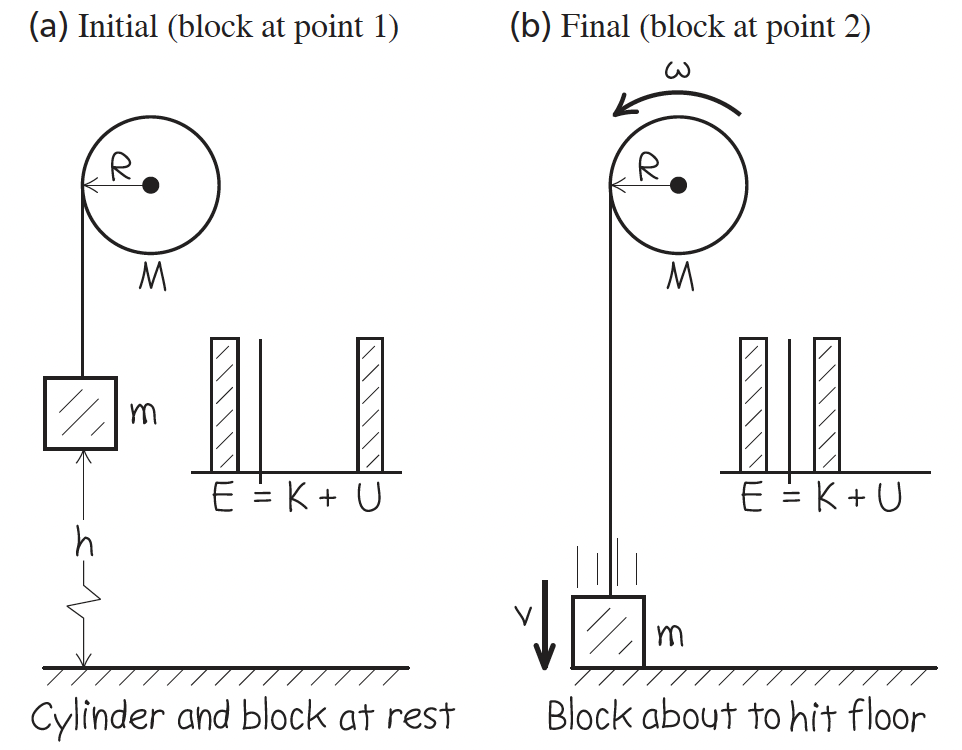
\includegraphics[width=0.5\linewidth]{../figures/9_17.png}
  \label{fig:9_17}
\end{figure}

In the system shown in (\textbf{\autoref{fig:9_17}}), a \qty{12,0}{kg} mass is released from rest and falls, causing the uniform \qty{10,0}{kg} cylinder of diameter \qty{30,0}{cm} to turn about a frictionless axle through its center. How far will the mass have to descend to give the cylinder \qty{480}{J} of kinetic energy
\bigbreak
Vi har, som vanligt, energikonservation
\[
k_1+U_1 = k_2 + U_2 \implies msg = \frac{1}{2}mv^2 + \frac{1}{2}\cdot \frac{1}{2}MR^2\omega^2 = \frac{1}{2}\left( m + \frac{1}{2}M \right) R^2\omega^2
.\] 
Det er i opgaven givet at $m = \qty{12,0}{kg}$ og at $M = \qty{10,0}{kg}$. Altså bliver forholdet mellem de to størrelser i parentesen
\[
\frac{m}{\frac{1}{2}M} = \frac{\qty{12,0}{kg}}{\frac{1}{2}\cdot \qty{10,0}{kg}} = \frac{12}{5}
.\] 
Og da det er oplyst at $k_M = \qty{480}{J}$ må det tilsvarende gælde at $k_m = \qty{480}{J}\cdot \frac{12}{5} = \qty{1152}{J}$. Altså har vi at
\[
k_{tot} = k_M + k_m = \qty{480}{J} + \qty{1152}{J} = \qty{1632}{J}
.\] 
Alt denne kinetiske energi må være omdannet potentiel energi $k_{tot} = msg \implies s = \frac{k_{tot}}{mg}$. Altså får vi at
\[
s = \frac{\qty{1632}{J}}{\qty{12,0}{kg}\cdot \qty{9,81}{\frac{m}{s^2}}} = \qty{13,86}{m}
.\] 

\section*{Opg. 9.89}

\begin{figure} [ht]
  \centering
  \caption{}
  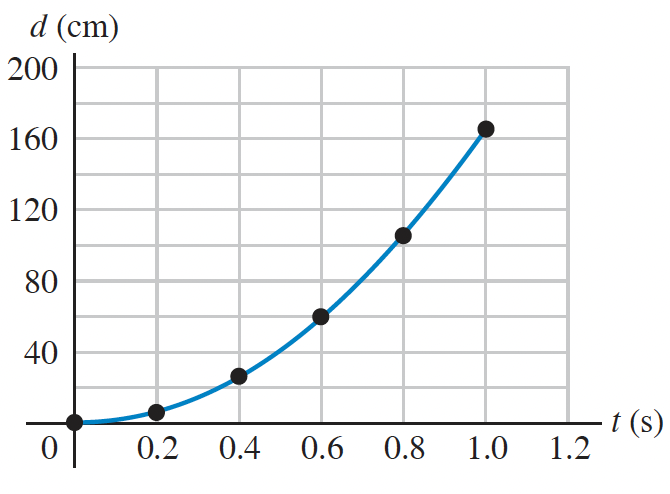
\includegraphics[width=0.5\linewidth]{../figures/P9_89.png}
  \label{fig:P9_89}
\end{figure}

You are rebuilding a 1965 Chevrolet. To decide whether to replace the flywheel with a newer, lighter-weight one, you want to determine the moment of inertia of the original, \qty{35,6}{cm}-diameter flywheel. It is not a uniform disk, so you can’t use $I = \frac{1}{2}MR^2$ to calculate the moment of inertia. You remove the flywheel from the car and use low-friction bearings to mount it on a horizontal, stationary rod that passes through the center of the flywheel, which can then rotate freely (about \qty{2}{m} above the ground). After gluing one end of a long piece of flexible fishing line to the rim of the flywheel, you wrap the line a number of turns around the rim and suspend a \qty{5,60}{kg} metal block from the free end of the line. When you release the block from rest, it descends as the flywheel rotates. With high-speed photography you measure the distance $d$ the block has moved downward as a function of the time since it was released. The equation for the graph shown in (\textbf{\autoref{fig:P9_89}}) that gives a good fit to the data points is $d = \left( \qty{165}{\frac{cm}{s^2}} \right)t^2$. 


\subsection*{(a)}
Based on the graph, does the block fall with constant acceleration? Explain.
\bigbreak
Afstanden som blokken har bevæget sig er givet ved
\[
d =\qty{165}{\frac{cm}{s^2}t^2} \text{, hvilet er på formen } d = \frac{1}{2}at^2
,\] 
så ja, blokken falder med konstant acceleration.


\subsection*{(b)}
Use the graph to calculate the speed of the block when it has descended \qty{1,50}{m}.
\bigbreak
Accelerationen af blokken er
\[
a = 2\cdot \qty{165}{\frac{cm}{s^2}} = \qty{3,30}{\frac{m}{s^2}}
.\]
Det gælder at $v^2 = as$. Altså har vi at
\[
v = \sqrt{2as} = \sqrt{2\cdot \qty{3,30}{\frac{m}{s^2}}\cdot \qty{1,50}{m}} = \qty{3,15}{\frac{m}{s}} 
.\] 


\subsection*{(c)}
Apply conservation of mechanical energy to the system of flywheel and block to calculate the moment of inertia of the flywheel.
\bigbreak
Energikonservation siger at
\[
k_1+U_1 = k_2+U_2 \implies msg = \frac{1}{2}mv^2 + \frac{1}{2}I\omega^2
.\] 
Og da det gælder at $\omega = \frac{v}{r}$ får vi at
\[
I = \frac{2R^2}{v^2} \left(msg - mv^2\right) = mR^2\left( \frac{2gs}{v^2} -1 \right) 
.\] 
Sættes alle kendte værdier ind i denne fås at
\[
I = \qty{5,60}{kg}\cdot (\qty{0,356}{m})^2 \left( \frac{2\cdot \qty{9,81}{\frac{m}{s^2}}\cdot \qty{1,50}{m}}{\left(\qty{3,15}{\frac{m}{s}}\right)^2} -1 \right) = \qty{1,40}{kg\cdot m^2}
.\] 
 


\subsection*{(d)}
You are relieved that the fishing line doesn’t break. Apply Newton’s second law to the block to find the tension in the line as the block descended.
\bigbreak
Vi har at
\[
gm + (-T) = ma \implies T = m(g-a) = \qty{5,60}{kg}\left( \qty{9,81}{\frac{m}{s^2}} - \qty{3,30}{\frac{m}{s^2}} \right) = \qty{36,456}{N}
.\] 
  

\end{document}
